\documentclass[a4,center,fleqn]{NAR}

% Enter dates of publication
\copyrightyear{2008}
\pubdate{31 July 2009}
\pubyear{2009}
\jvolume{37}
\jissue{12}

%\articlesubtype{This is the article type (optional)}

\begin{document}

\title{\textit{dpcR} a Swiss-army knife for the analysis of digital PCR experiments}

\author{%
Micha\l{} Burdukiewicz\,$^{1,5}$,
Jim Huggett\,$^{2}$,
Alexandra Whale\,$^{2}$,
Bart K.M. Jacobs\,$^{3}$,
Lieven Clement\,$^{3}$,
Piotr Sobczyk\,$^{1}$,
Andrej-Nikolai Spiess\,$^{4}$,
Peter Schierack\,$^{5}$,
Stefan R\"odiger\,$^{5,}$\footnote{To whom correspondence should be addressed.
Tel: +49 357385936; Fax: +49 357385801; Email: stefan.roediger@b-tu.de}}

\address{%
$^{1}$Department of Genomics, Faculty of Biotechnology, University of Wroc\l{}aw, Wroc\l{}aw, Poland
and
$^{2}$Molecular and Cell Biology Team, LGC, Teddington, United Kingdom
and
$^{3}$Department of Applied Mathematics, Computer Science and Statistics, Ghent University, Belgium
and
$^{4}$University Medical Center Hamburg-Eppendorf, Hamburg, Germany
and
$^{5}$Faculty of Natural Sciences, Brandenburg University of Technology Cottbus--Senftenberg, Gro\ss{}enhainer Str. 57, 01968, Senftenberg, Germany
}
% Affiliation must include:
% Department name, institution name, full road and district address,
% state, Zip or postal code, country

\history{%
Received January 1, 2009;
Revised February 1, 2009;
Accepted March 1, 2009}

\maketitle

\begin{abstract}

The digital Polymerase Chain Reaction (dPCR) is emerging in all research areas, 
such as life-sciences and diagnostics since it enables an absolute 
quantification of nucleic acids. Different approaches for statistical analysis 
were proposed. However, most analysis is done in closed source software as 
provided by the vendors. This makes it harder to compare results, such as the 
confidence interval estimates. An unified open software framework for 
reproducible research is not available.

To perform dPCR analysis we implemented peer-review statistical methods and 
plots into the \textit{dpcR} framework, based on the sophisticated statistical 
computing environment \textbf{R}. \textit{dpcR} is versatile open source 
cross-platform software framework, which provides functions to process dPCR data 
independent of the hardware. Our software can be used for data analysis and 
presentation, as framework for novel technical developments and as reference for 
statistical methods in dPCR analysis. Features such as functions to estimate the 
underlying Poisson process, calculation of confidence intervals based on single 
samples as well as on replicates, a novel Generalized Linear Model-based 
procedure to compare digital PCR experiments and a spatial randomness test for 
assessing plate effects have been integrated. We use a plug-in like architecture 
and abstraction layers to make the framework usable for droplets and (real-time) 
chamber based technologies.

\textit{dpcR} was implemented with interfaces to the command-line, graphical 
user interfaces and interactive web application. \textit{dpcR} can be used by 
novices in a graphical user interface or by experts via a command-line 
interface. The \textit{dpcR} framework can be used to build a custom-made 
analyser according to the wishes of the user. The \textit{dpcR} framework is an 
open environment, which can be adopted to the growing knowledge in dPCR. 

\end{abstract}


\section{Introduction}

Real-time quantitative PCR (qPCR) is the standard approach to quantify nucleic 
acids \cite{pabinger_survey_2014}. The quantification of the amplification is 
not done by determining a Cq-value derived from an amplification curve. qPCR is 
a well established and robust technology, which allows precise quantification of 
DNA material in high throughput fashion. However, the quantification by qPCR is 
challenging at very low and very high concentrations. At low DNA concentration 
Monte Carlo effect play a role and at high concentration inhibition processes 
start to dominate the qPCR. Thus, the qPCR is only usable in the working range 
of the calibrator. In addition, pre-processing and data analysis is a affected 
by numerous adverse effects \cite{ruijter_2013, spiess_impact_2015}.


The digital PCR (dPCR) is an alternative method to quantify nucleic acids. The 
chemical basis of the dPCR is similar to the qPCR, which includes master-mix 
preparation and thermal cycling of the sample. In contrast to qPCR the 
amplification reaction does not take place in a single reaction chamber. Rather 
its a process of clonal amplification in small separate ``partitions'' (e.g., nl 
volume droplets of water oil emulsions, chambers on micro structured chips). The 
number of positive partition in relation to the number of total partitions. By 
applying Poisson statistics it is possible to determine the number of the 
starting material in given volume. Therefore, the dPCR does not require an 
external calibration \cite{selck_increased_2013, rodiger_r_2015}. Since 
approximately ten years the digital PCR (dPCR) is gaining momentum in the 
mainstream user-base. dPCR will likely have the same impact as qPCR in the 
nucleic acid methodology \cite{huggett_qpcr_2015, morley_digital_2014, 
rodiger_r_2015}. There is an intensive research on dPCR platforms with the 
overall aim to make to technology broadly usable, cheap, robust and to enable 
high sample throughput.

% **************************************************************
% Keep this command to avoid text of first page running into the
% first page footnotes
\enlargethispage{-65.1pt}
% **************************************************************

A first proposal for digital PCR like approach and the use of the Poisson 
distribution to quantify the number of molecules on a ``sample'' was shown by 
Ruano \textit{et al.} 1990 (PNAS) with the single molecule dilution (SMD) PCR \cite{ruano_haplotype_1990}. In 1999 
Vogelstein \textit{et al.} (PNAS) described the first true digital PCR \cite{vogelstein_digital_1999}. Application of 
the dPCR cover all applications of conventional qPCR, including investigation of 
alleles, gene expression analysis and absolute quantification of PCR products. 
For absolute quantification the qPCR relied on an external calibrator 
(calibration curve) which was derived serial decadic dilution (e.g., 1:10 $\rightarrow$ 
1:100 $\rightarrow$ 1:1000) of a known target input quantity. The real-time monitoring of 
the PCR product formation enabled to determine quantification points (Cq). The 
Cq are strictly related to the input quantity. A simple arithmetic operation 
(after logarithmic transformation of the concentration) is sufficient to 
determine any nucleic acid quantity \cite{huggett_considerations_2014}.

qPCR	dPCR
Number of copies/DNA per volume (e.g., ng/µl, copies/µl)	total number of compartments * ln (...)

The dPCR has some principle assumptions and fundamental properties. First of all 
the chemical reaction should be not affected by inhibitors. The distribution of 
the single molecule target regions follows a Poission distribution. The Poisson 
distribution appears like a normal distribution but without negative values and 
being zero the lowest. First a large number (n) of amplifications reactions as 
required to have a high statistical power. Therefore in practical terms a 
massive number of PCR reactions is needed. For Poission distributions an n of XY 
(get reference from table/text book form statistics/biostatistics?) is 
considered large. Second that the molecules required for the amplification 
amplifications reactions are randomly distributed in the compartments. Visual 
analysis, Ripley's K functions or ??? can be used to test for randomness of the 
reaction and thus to exclude the clustering of of positive reactions. A 
clustering of positive wells might be due to sample loading or analysis process 
(systematical error). The outcome of an amplification can be no amplification at 
all (less than 1 copy per volume), an unsaturated reaction with a 
binary/``multinary'' amplification (usable to calculate the ``concentration'') 
or a saturated reaction where virtually all compartments are positive.

Calculation of the ``Concentration''
Reference to ``Supplement''

Calculation of the uncertainty
To determine the uncertainty of the calculations two approach have been proposed 
in the peer-review literature \cite{dube_mathematical_2008, bhat_single_2009}. The uncertainty is 
dependent on the number of PCR reactions (reference to \textit{\textit{dpcR}} 
functions). … Reference to ``Supplement'' and \textit{dpcR} functions.



Interactive use and graphical representation with \textit{shiny} \cite{shiny}.

Import and export of results figures and data.

There are currently two technical approaches to dPCR. dPCRs may use		%  (e.g., QuantStudio$\circledR$ 12K Flex (Life Technologies), BioMark\texttrademarkTM  EP1TM (Fluidigm))
(microfluidic)chambers or emulsion based chambers 
(QX200 \texttrademark (Bio-Rad), RainDrop \texttrademark System (RainDance)). 
Chamber based dPCR systems have fixed geometries, including the volume of the 
reaction chambers. Despite the fact that dPCRs is an endpoint analysis the 
chamber based technologies allow generally the real-time monitoring of the 
amplification reaction and subsequent confirmation of the amplification reaction 
be melting curve analysis. Thus, such technologies enable easier trouble 
shooting and quality management of the data. However, the downside of these 
technologies is the fixed limited number of compartments and the price. The 
emulsion based dPCRs are easier to perform since the compartments are generated 
by microfluidic technologies and have practically no limitation regarding the 
number of compartments. This results in a higher statistical power to quantify 
small differences in sample quantities. The emulsion chambers are made of 
water-in-oil emulsions with similar sizes.


Two-sided exact tests and matching confidence intervals for discrete data \cite{fay_2010}

Controlling the False Discovery Rate: A Practical and Powerful Approach to Multiple Testing \cite{benjamini_1995}

Interval Estimation for a Binomial Proportion \cite{brown_2001}

There is a need for an vendor independent data analysis. For example others 
\cite{strain_highly_2013} have written task custom software for data analysis in 
\textbf{Mathematica} (Wolfram Research). However, we have chosen \textbf{R} 
because it is the \textit{lingua franca} in biostatistics and broadly used in 
other disciplines \cite{rodiger_r_2015}. The are many packages in existence 
which enable the fast development of new methods and plotting facilities. As 
most \textbf{R} packages depend on one or more other packages \cite{ooms_2013} 
depends \textit{dpcR} on other packages, resulting in a complex network of 
recursive dependencies. Core packages \textit{qpcR} \cite{ritz_qpcr_2008}, 
\textit{shiny} \cite{shiny}, \textit{MBmca} \cite{rodiger_surface_2013}, 
\textit{chipPCR} \cite{rodiger_chippcr_2015} and further packages as shown in 
the dependency graph (Supplement XYZ).

 

\textbf{R} has a rich set of tool to arrange data (reshape?) in order to prepare them for 
the analysis. This is important when it comes to the question how experiments 
should be treated. It is possible to analyze the PCR reaction the panels 
independently (effect on CI and uncertainty) or to pool/aggregate all reactions 
(effect on CI and uncertainty) to achieve higher sensitivity/certainty.

% **************************************************************
% Keep this command to avoid text of first page running into the
% first page footnotes
\enlargethispage{-65.1pt}
% **************************************************************


\section{MATERIALS AND METHODS}

\subsection{Materials subsection one}

One basic design decision was to structure specific properties of digital PCR 
systems (dropet vs. chamber) in auxiliary functions and to perform central 
calculation specific to Poisson statistics in independent main functions. 
Chamber digital PCR systems fundamentally rely on the proper preprocessing of 
qPCR data. We have chosen to implement the core functionality by a dependency to 
the \textit{qpcR} \textbf{R} package \cite{ritz_qpcr_2008}. The main functions (e.g., for analysis, 
simulations, plotting), several auxiliary helper functions (e.g., data import) 
and data set of different dPCR systems are listed in Table XY. Further 
dependencies to 3rd party packages include \textit{pracma}, ... (see Figure \ref{dpcR_implementation_1}). See the vignette for 
details.

The workflow is shown Figure \ref{workflow}.

\begin{figure*}[t]
\begin{center}
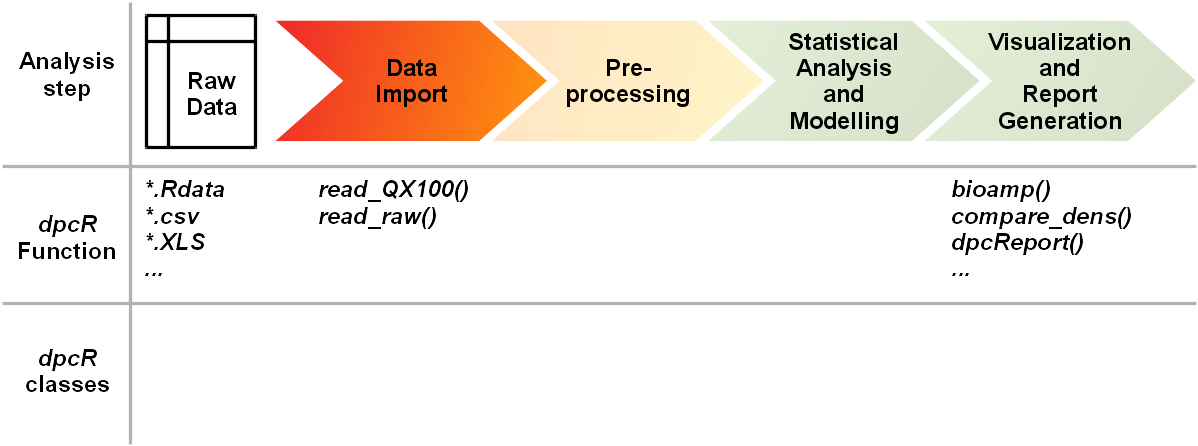
\includegraphics[width=17cm]{workflow.png}
\end{center}
\caption{\textit{dpcR} workflow. Show steps in dPCR data analysis.} 
\label{workflow}
\end{figure*}

The GUI employs advanced plots based on \textit{ggplot2} \cite{kahle_wickham_2013}.

\begin{figure}[t]
\begin{center}
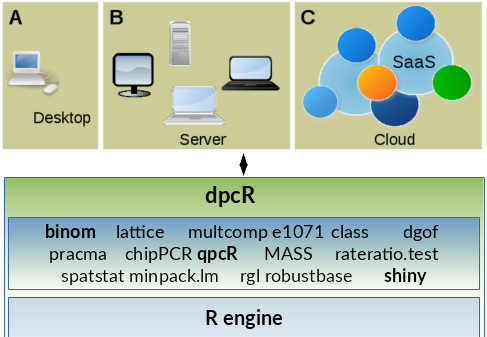
\includegraphics[width=9cm]{dpcR_implementation_1.png}
\end{center}
\caption{Modular software framework structure. \textit{dpcR} is typically run from a 
desktop computer or a server. The software can be operated by an GUI/IDE 
application such as \textbf{RStudio} or \textbf{RKWard}. The \textit{dpcR} 
package has dependencies to other \textbf{R} packages (middle layer). The 
functionality shared between the packages enables repaid addition and expansion 
of functionality.} 
\label{dpcR_implementation_1}
\end{figure}

\begin{figure}[t]
\begin{center}
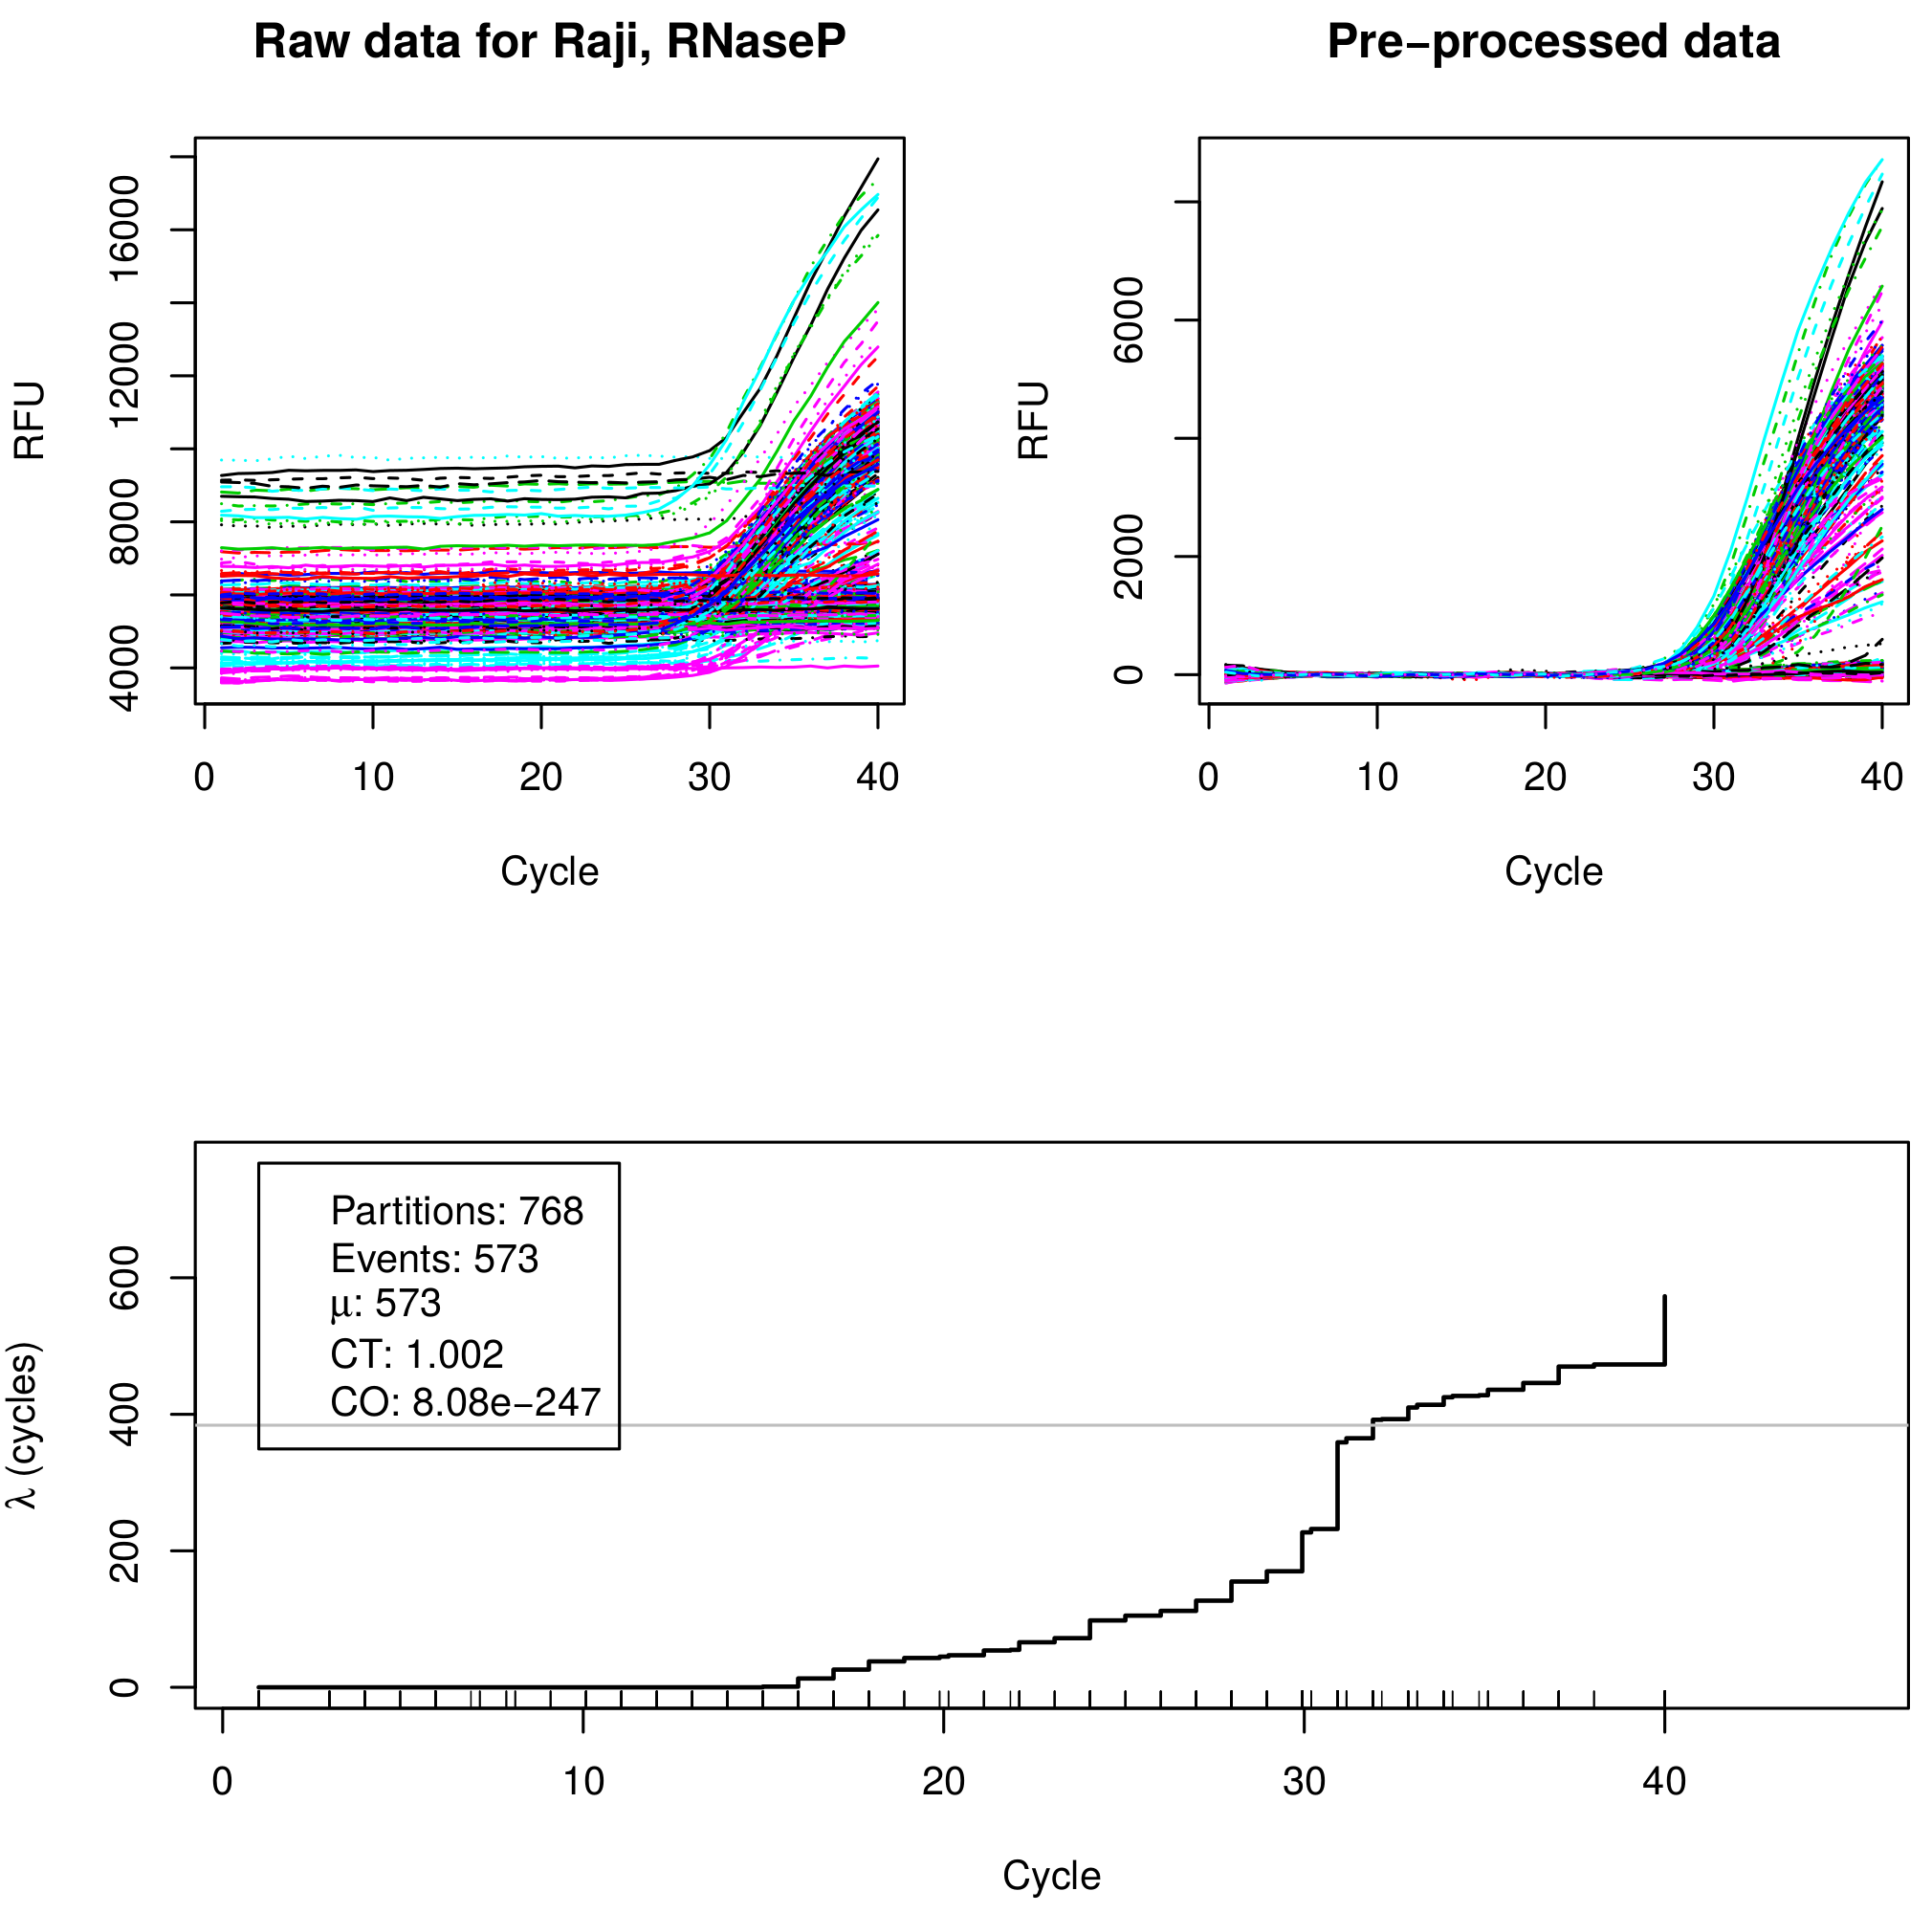
\includegraphics[width=9cm]{qpcr2pp_1.png}
\end{center}
\caption{Uncover characteristics of dPCR data with the \textit{dpcR} and \textit{chipPCR} packages. 
Selected dPCR platforms are real-time platforms. The function \textit{qpcr2pp} uses the 
real-time data and interprets them as dPCR (Poisson process). A) Raw data of The 
function were B) preprocessed (baselined, smoothed) with functions from the 
\textit{chipPCR} package and C) finally analyzed (Cq calculation $\rightarrow$ binarize) with the 
\textit{qpcr2pp} (qPCR to Poisson process) function from the \textit{dpcR} package.} 
\label{dpcR_implementation_1}
\end{figure}

\subsubsection{Materials subsubsection one.}

\begin{align}
\mathrm{LD}^r = \frac{\mathrm{LD}}{A_\mathrm{iso}}
= 1.5 S \left( 3 \cos^2 \alpha_i - 1 \right)
\end{align}



\subsection{Materials subsection two}

We aimed for a form factor (e.g., smart phone, tablet, desktop PCR) and 
operating system independent implementation of a graphical user interface. 

Moreover, there exit several GUI technologies for \textbf{R} \cite{rodiger_rkward_2012}.
(see Figure \ref{GUI_RKWard_1}).

Text.

\begin{equation*}
\mathrm{LD} \left( t \right) =
\sum\limits_i
a_i \exp \left( \frac{-t}{\tau_i} \right)
\end{equation*}

Text.

\begin{figure*}[t]
\begin{center}
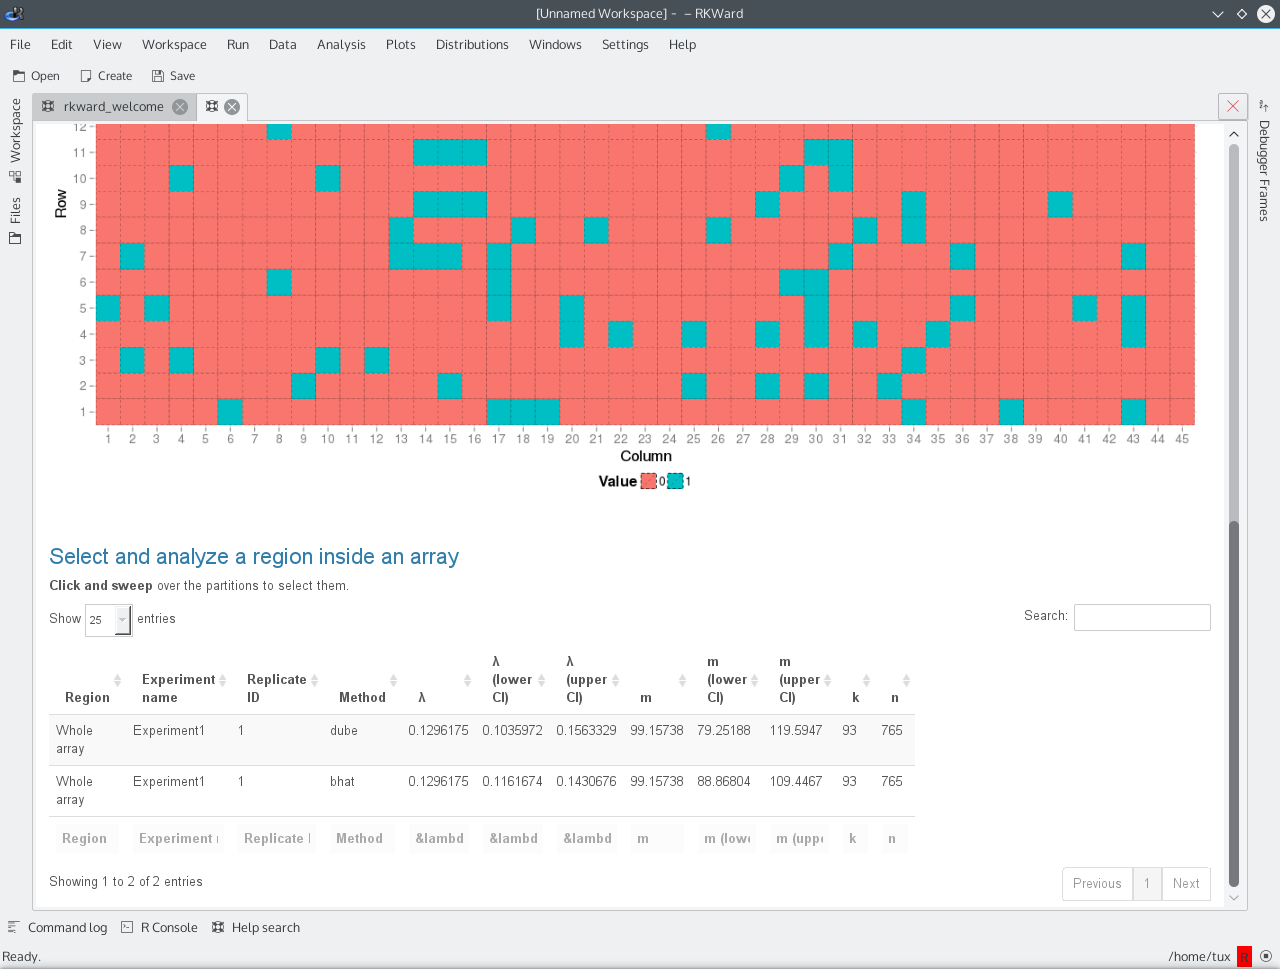
\includegraphics[width=17cm]{GUI_RKWard_1.png}
\end{center}
\caption{\textit{dpcrReport()} function running in the graphical user interface and integrated development environment \textbf{RKWard}.}
\label{GUI_RKWard_1}
\end{figure*}

\subsection{Materials subsection Statistical power - Monte Carlo simulations}

The proposed framework was evaluated in three Monte Carlo experiments (2000 times repetitions each) with accordingly 1000, 5000 (results not shown) and 10k partitions. During each repetition of the Monte Carlo scheme, a set of partitions was randomly generated~\cite{dube_mathematical_2008} with a determined number of molecules ('Base number of molecules' on X-axis). The set was copied and a number of molecules ('Added number of molecules' on Y-axis) was added to randomly chosen partitions. Two obtained arrays were compared using the proposed method. The mean p-values alongside with their standard deviation are presented in the chart below.

\begin{figure}[t]
\begin{center}
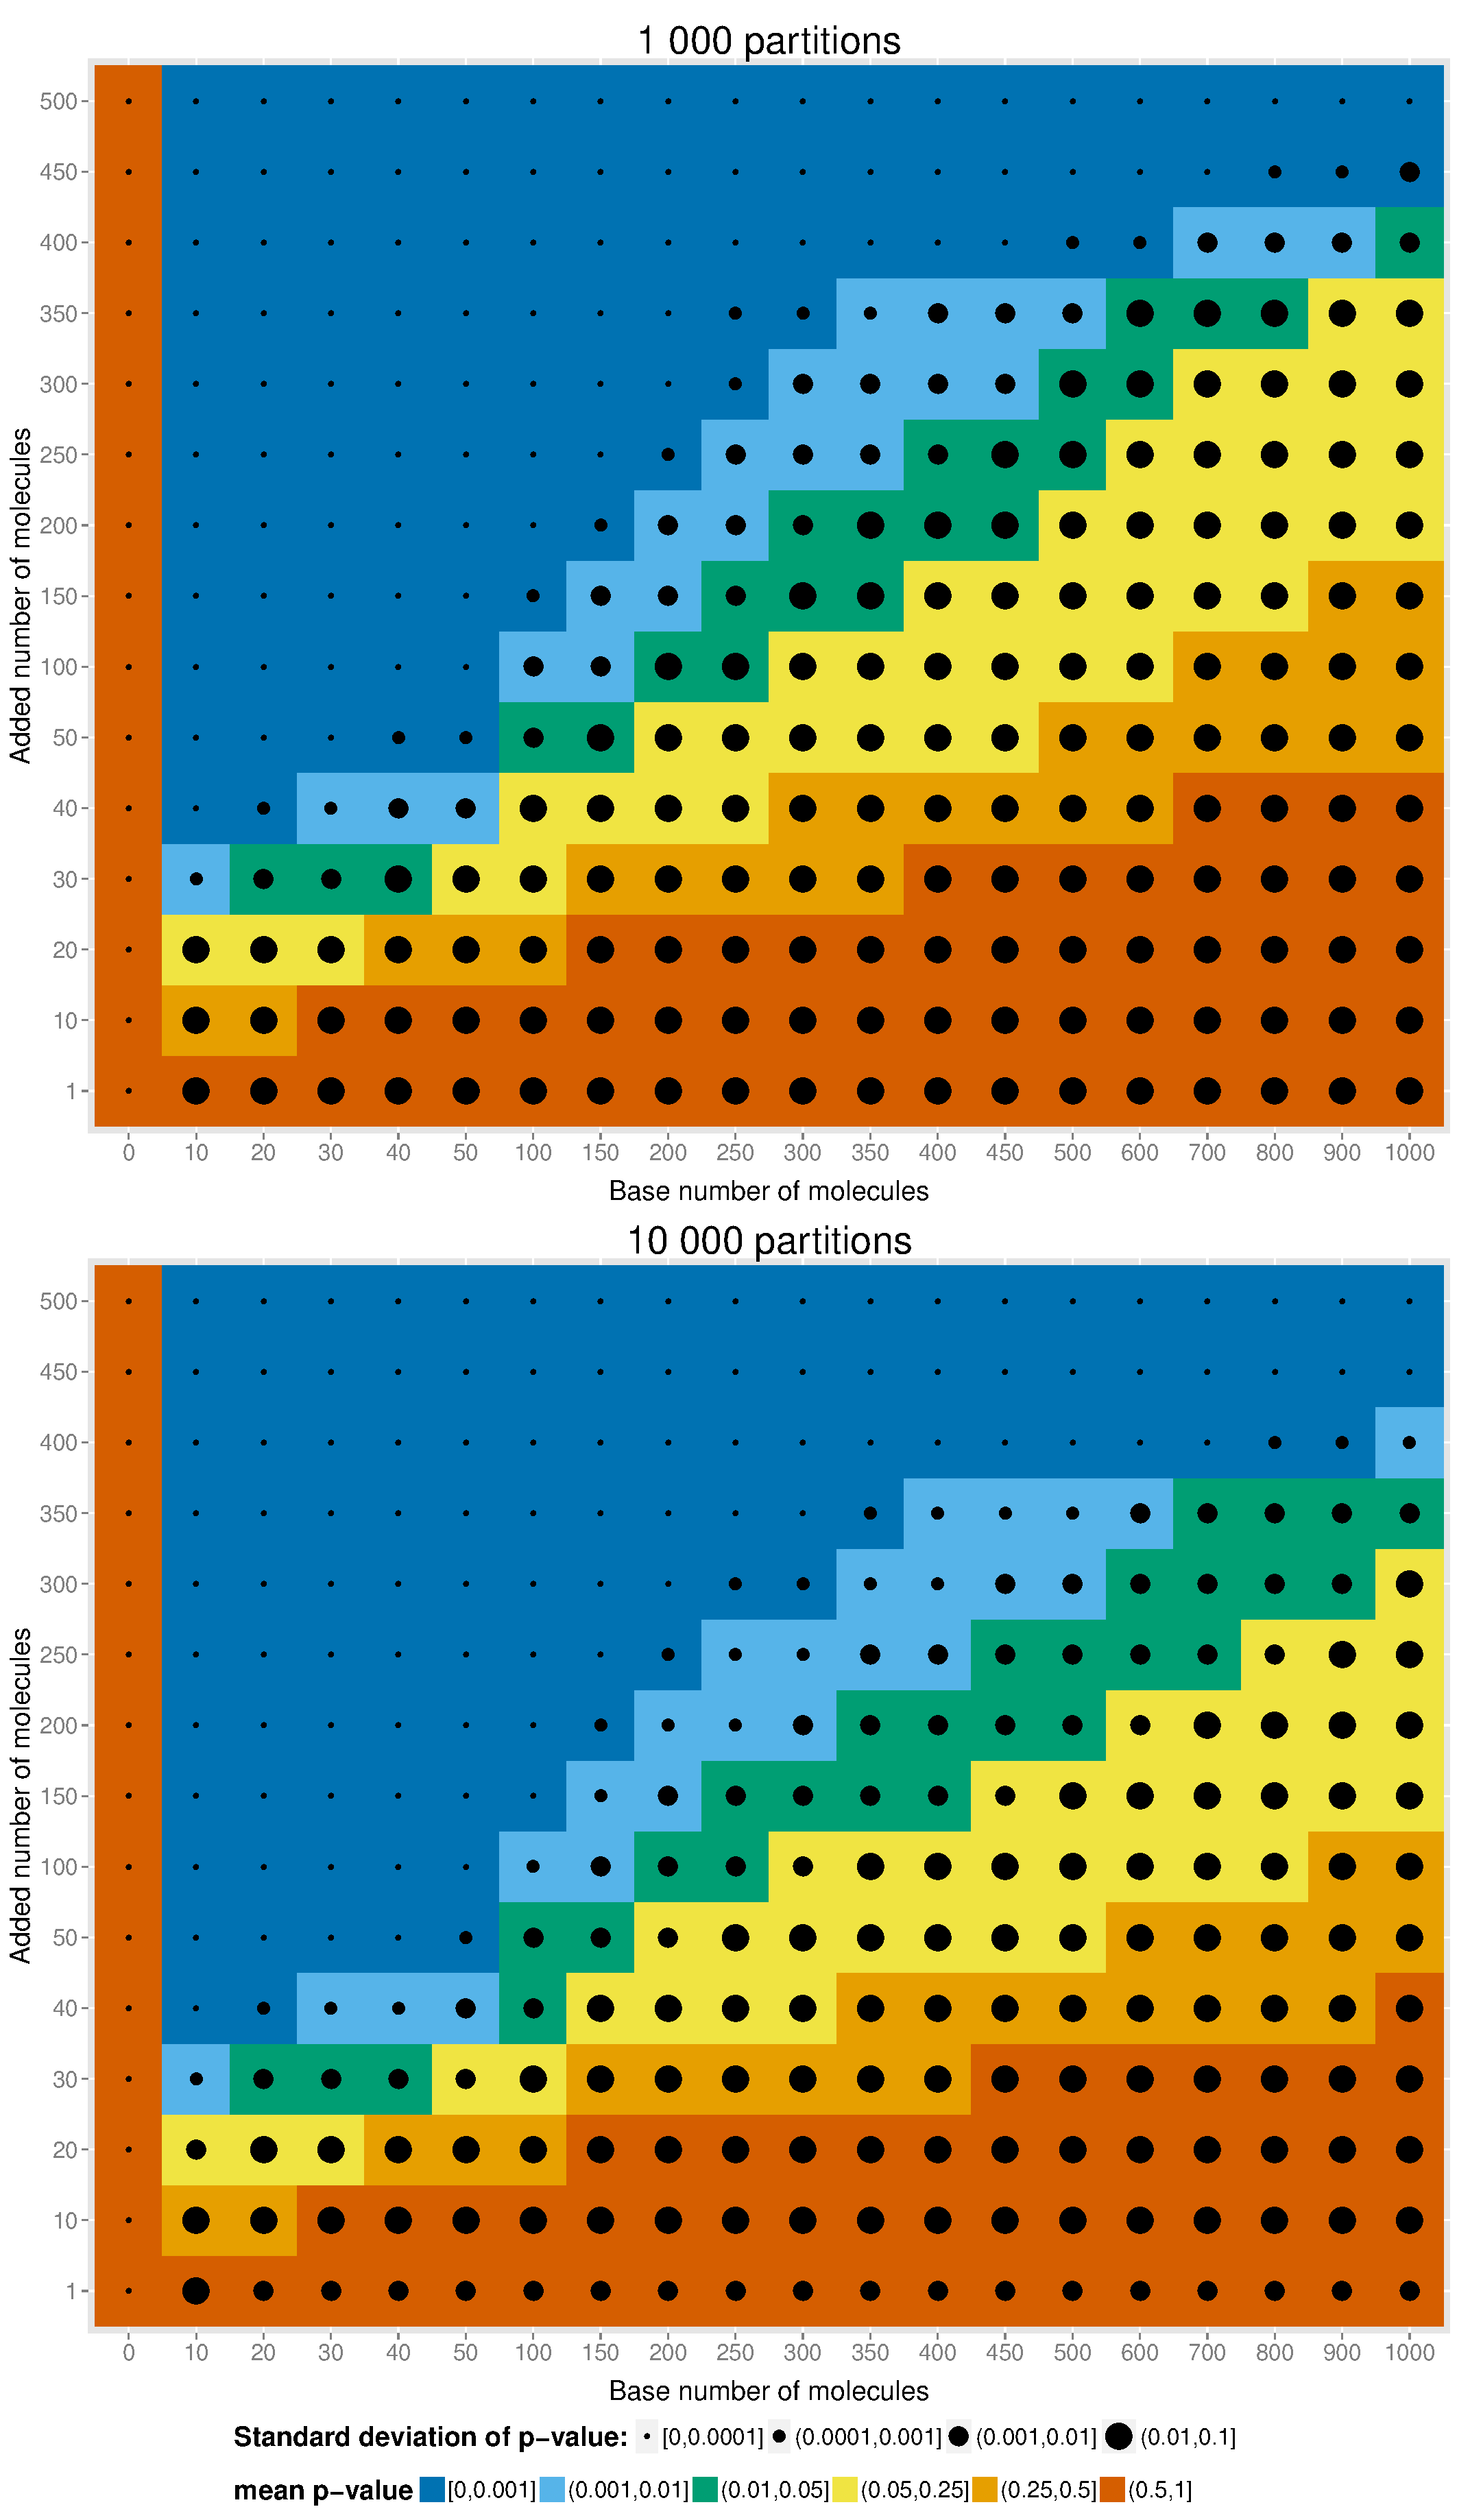
\includegraphics[width=9cm]{mc_figures-1.pdf}
\end{center}
\caption{Our method, based on GLM, predicts estimated means copies per partitions using Poisson or binomial regression. Afterwards, estimates are compared against themselves using t-test. Obtained p-values and confidence intervals do not require further correction, because the familywise error is controlled through the whole analysis.}
\label{mc_figures-1}
\end{figure}

\section{RESULTS}

\subsection{Reading or importing data}

(see Table \ref{table_formats}).

\begin{table}[b]
\tableparts{%
\caption{Structured export data formats handled by \textit{dpcR}~v.~0.5 and later.}
\label{table_formats}%
}{%
\begin{tabular*}{\columnwidth}{@{}llll@{}}
\toprule
Vendor & System & Format & Type
\\
\colrule
Bio-Rad & QX100 \& QX200 & CSV & Summary export
\\
Fluidigm & BioMark & CSV & Summary export
\\
Formulatrix & Constellation Digital PCR & CSV & Summary export
\\
\botrule
\end{tabular*}%
}
{The number of structured export data formats handled by \textit{dpcR} is growing. Numerous data 
formats can be processed with the functionality provided by the \textbf{R} 
environment (see \cite{rodiger_r_2015}). CSV, comma separated values.
} \end{table}

\subsection{Public data sets}

\textit{dpcR} includes data sets or refers to additional R packages for testing 
purposes. The data originate from different dPCR and qPCR systems and were 
either published previously \cite{whale_comparison_2012, 
rodiger_chippcr_2015,rodiger_r_2015} or \textit{de novo} generated.

\subsection{Results subsection two}
  
(see Table \ref{table_formats}).


\subsection{Availability}

The \textit{dpcR} framework is available as open source software package as part 
of the Bioconductor project \cite{gentleman_2004}. The source code is open 
source (GPL-3 or later). The stable version is hosted at 
http://cran.r-project.org/web/packages/dpcR and the source code is available 
from  https://github.com/michbur/dpcR.

\subsection{Documentation}

All functions of the \textit{dpcR} package have its own documentation package, 
which specifies the input types, classes, parameters and output formats.

\section{DISCUSSION}

We developed the \textit{dpcR} package, which is a software framework for analysis of 
dPCR based on the open source statistical software \textbf{R}. \textit{dpcR} provides the scientific 
community a broadly applicable tool for teaching purposes, data analysis and theoretical research based on simulations. 

To accelerate the development of new approaches to dPCR. 

We implemented all existing statistical methods for dPCR and suggest the 
introduction of a standardized nomenclature for qPCR. The package enables the 
simulations and predictions of Poisson distribution for dPCR scenarios, the 
analysis of previously run dPCRs.

Functions included may be used to simulate dPCRs, perform statistical data 
analysis, plotting of the results and simple report generation. 

There are currently different software solutions for dPCR analysis such as the 
OpenArray software (Life Technologies) or XYZ (Bio-Rad). Most of the are black 
boxes which prevent deep insight into the data processing step. In addition most 
of the software solutions are aimed to be used in very specific scenarios and a 
mutual exclusive to alternative platforms (e.g., droplet vs. chamber-based). We 
have chosen \textbf{R} because it is the \textit{lingua franca} in biostatistics and broadly used 
in other disciplines \cite{rodiger_r_2015}.

\subsection{Discussion subsection one}

Text.


\subsection{Discussion subsection two}

Text.


\subsection{Discussion subsection three}


\section{CONCLUSION}

In conclusion, \textit{dpcR} provides means to understand how digital PCR works, 
to design, simulate and analyze experiments, and to verify their results (e.g., 
confidence interval estimation), which should ultimately improve 
reproducibility. We have built what we believe to be the first unified, 
cross-platform, dMIQE compliant, open source (GPL-3 or later) software framework for 
analyzing digital PCR experiments. Our framework, designated \textit{dpcR} , is 
targeted at a broad user base including end users in clinics, academics, 
developers, and educators. We implemented existing statistical methods for dPCR 
and suggest the introduction of a standardized nomenclature for qPCR. Our 
framework is suitable for teaching and includes references for an elaborated 
set of methods for dPCR statistics. Our software can be used for (I) data 
analysis and visualization in research, (II) as software framework for novel 
technical developments, (III) as platform for teaching this new technology and 
(IV) as reference for statistical methods with a standardized nomenclature for 
dPCR experiments. The framework enables the simulations and predictions of Poisson 
distribution for dPCR scenarios, the analysis of previously run dPCRs. Due to 
the plug-in structure of the software it is possible to build custom-made 
analyzers.

The \textit{dpcR} includes 
to invitation to the scientific community to join and support the development of 
\textit{dpcR} (github?).


\section{ACKNOWLEDGEMENTS}

Grateful thanks belong to the \textbf{R} community.

\section{Funding}
This work was funded by the Federal Ministry of Education and Research (BMBF) InnoProfile--Transfer--Projekt 03 IPT 611X.
 
\subsubsection{Conflict of interest statement.} None declared.
\newpage


\bibliographystyle{plain}
\bibliography{dpcr}
\end{document}
